\documentclass[UTF8,a4paper]{article}
\usepackage{fancyhdr}
\usepackage{ctex}
\usepackage{amsmath}
\usepackage{listings}
\usepackage{color}
\usepackage{graphics}
\usepackage{graphicx}
\lstset{ %
	extendedchars=false,            % Shutdown no-ASCII compatible
	language=Matlab,                % choose the language of the code
	basicstyle=\small\sf,    % the size of the fonts that are used for the code
	tabsize=3,                            % sets default tabsize to 3 spaces
	numbers=left,                   % where to put the line-numbers
	numberstyle=\tiny,              % the size of the fonts that are used for the line-numbers
	stepnumber=1,                   % the step between two line-numbers. If it's 1 each line
	% will be numbered
	numbersep=5pt,                  % how far the line-numbers are from the code   %
	keywordstyle=\color[RGB]{33,33,234},               % keywords
	commentstyle=\color[RGB]{0,0,0},    % comments
	stringstyle=\color[rgb]{0.170,0.187,0.102},      % strings
	backgroundcolor=\color{white}, % choose the background color. You must add \usepackage{color}
	showspaces=false,               % show spaces adding particular underscores
	showstringspaces=false,         % underline spaces within strings
	showtabs=false,                 % show tabs within strings adding particular underscores                frame = single,         % adds a frame around the code
	captionpos=b,                   % sets the caption-position to bottom
	breaklines=true,                % sets automatic line breaking
	breakatwhitespace=false,        % sets if automatic breaks should only happen at whitespace
	title=\lstname,                 % show the filename of files included with \lstinputlisting;
	% also try caption instead of title
	mathescape=true,escapechar=?    % escape to latex with ?..?
	escapeinside={\%*}{*)},         % if you want to add a comment within your code
	%columns=fixed,                  % nice spacing
	%morestring=[m]',                % strings
	%morekeywords={%,...},%          % if you want to add more keywords to the set
	%    break,case,catch,continue,elseif,else,end,for,function,global,%
	%    if,otherwise,persistent,return,switch,try,while,...},%
}
\pagestyle{fancy}
\lhead{}
\chead{}
\rhead{\bfseries The Matlab $5^{th}$ Homework week 7}
\lfoot{}
\cfoot{\thepage}
\rfoot{}
\renewcommand{\headrulewidth}{0.4pt}
\begin{document}
\begin{center}
    \textbf{\LARGE{Matlab $5^{th}$ Homework week 7}}\\[0.5cm]
    \normalsize{庄震丰 22920182204393}\\[0.5cm]
    \large{Oct. $31^{th}$, 2019}
\end{center}
\section{Limit}
\subsection{Description}
 
$$
\begin{aligned}
    &lim_{x \rightarrow a} \frac{sinx-sina}{x-a}\\
    &lim_{x\rightarrow \infty} (\frac{2x+3}{2x+1})^{x+1}\\
    &lim_{x\rightarrow a^{+}} \frac{\sqrt{x}-\sqrt{a}+\sqrt{x-a}}{\sqrt{x^2-a^2}}\\
    &lim_{x\rightarrow a^{-}} \frac{\sqrt{x}-\sqrt{a}+\sqrt{x-a}}{\sqrt{x^2-a^2}}\\
    &lim_{x\rightarrow 0} \frac{tan(2x)}{tan(5x)}
\end{aligned}
$$
\subsection{Analysis}
\noindent Solve the problem by useing \textit{limit} function.\\
Limit(f,variable,value,'left' or 'right').
\subsection{Codes and Result}
\textbf{Question 1}
\begin{lstlisting}
    syms x a;
    f=(sin(x)-sin(a))/(x-a);
    limit(f,x,a)
\end{lstlisting}
\textbf{Result}\\
ans=cos(a)\\\\
\textbf{Question 2}\\
\begin{lstlisting}
    syms x;
    f=((2*x+3)/(2*x+1))^(x+1);
    limit(f,x,inf)
\end{lstlisting}
\textbf{Result}\\
ans=exp(1)\\\\
\textbf{Question 3}
\begin{lstlisting}
    syms x a;
    f=(sqrt(x)-sqrt(a)+sqrt(x-a))/sqrt(x^2-a^2);
    limit(f,x,a,'right')    
\end{lstlisting}
\textbf{Result}\\
$ans =\frac{1}{\sqrt{2a}}$\\\\
\textbf{Question 5}\\
\begin{lstlisting}
    syms x a;
    f=(sqrt(x)-sqrt(a)+sqrt(x-a))/sqrt(x^2-a^2);
    limit(f,x,a,'left')
\end{lstlisting}
\textbf{Result}\\
$ans =\frac{i}{\sqrt{-2a}}$\\\\
\textbf{Question 4}\\
\begin{lstlisting}
    syms x;
    f=tan(2*x)/tan(5*x);
    limit(f,x,0)    
\end{lstlisting}
\textbf{Result}\\
ans =2/5\\\\

\section{Differential}
\subsection{Description}
\begin{center}
{f}={t} sin(x)\\
\end{center}
$$
solve~~~\frac{df}{dx},\frac{df}{dt},\frac{d^2f}{dxdt}
$$
\begin{center}
    ${f}=x^{y^z}$\\
\end{center}
$$
solve~~~\frac{\partial f}{\partial x},\frac{\partial f}{\partial y},\frac{\partial f}{\partial z}
$$
\subsection{Anaylsis}
\noindent use function \textit{diff} to get Differential number.\\
diff(f,variable~x,steps~n).
\subsection{Code and Result}
\textbf{Question 1}\\
\begin{lstlisting}
    syms t x;
    f=t*sin(x);
    diff(f,x)
    diff(f,t)
    diff(diff(f,x),t)       
\end{lstlisting}
\textbf{Result}\\
ans=x*cos(x)\\
ans=sin(x)\\
ans=cos(x)\\\\
\textbf{Question 2}\\
\begin{lstlisting}
    syms x y z;
    f=x^(y^z);
    diff(f,x)
    diff(f,y)
    diff(f,z)\end{lstlisting}
\textbf{Result}\\
ans =x\^(y\^z - 1)*y\^z\\
ans =x\^(y\^ z)*y\^ (z - 1)*z*log(x)\\
ans =x\^(y\^ z)*y\^ z*log(x)*log(y)\\\\
\section{Solve INT}
\subsection{Description}
$$
\begin{aligned}
    I&=\int_{0}^{2\pi}d\alpha \int_{0}^{\frac{pi}{4}} d\theta \int_{0}^{2acos\theta} r^2(1+cos\theta)sin\theta dr\\
    I&=\int_{-\infty}^{+\infty} \frac{1}{1+x^2} dx
\end{aligned}
$$
\subsection{Anaylsis}
\noindent Use function int(f,x,a,b)
\subsection{Code and Result}
\textbf{Question 1}\\
\begin{lstlisting}
    syms u theta r a;
    f=r^2*(1+cos(u))*sin(theta);
    int(int(int(f,r,0,2*a*cos(theta)),theta,0,pi/4),u,0,2*pi)    
\end{lstlisting}
\textbf{Result}\\
ans=pi*$a^3$\\\\
\textbf{Question 2}\\
\begin{lstlisting}
    clear all;
    syms x;
    f=1/(1+x^2);
    int(f,x,-inf,inf)    
\end{lstlisting}
\textbf{Result}\\
ans=pi\\\\
\section{Equations}
\subsection{Description}
$$
    \left\{  
        \begin{aligned}  
        x(x+y+z)&=a\\
        y(x+y+z)&=b\\
        z(x+y+z)&=c        
        \end{aligned}  
    \right.  
$$  
When a=16,b=12,c=18,solve x,y,z.
\subsection{Anaylsis}
\noindent In MATLAB, the solve() function can solve Equations,which automatically give the Results of the syms. 
\subsection{Code and Result}
\begin{lstlisting}
    syms x y z;
    a=16;
    b=12;
    c=18;
    equ1=x*(x+y+z)-a;
    equ2=y*(x+y+z)-b;
    equ3=z*(x+y+z)-c;
    s=solve(equ1,equ2,equ3,x,y,z);
    s.x
    s.y
    s.z    
\end{lstlisting}
\textbf{Result}\\
$$
    \left\{
    \begin{aligned}
    x1=-(8*46^{1/2})/23\\
    y1=-(6*46^{1/2})/23\\
    z1=-(9*46^{1/2})/23\\
    \end{aligned}
\right.
$$
$$
    \left\{
    \begin{aligned}
    x1=(8*46^{1/2})/23\\
    y1=(6*46^{1/2})/23\\
    z1=(9*46^{1/2})/23\\
    \end{aligned}
\right.
$$
\section{Non-Homogenous Differential Equation}
\subsection{Description}
$$
\frac{d^2y}{dx^2}-5\frac{dy}{dx}+6y=xe^{2x}
$$
\noindent To find the general solution of the non-homogenous differential equation of the second-order constant coefficient.
\subsection{Anaylsis}
\noindent use function \textit{dsolve} to get the solution of the non-homogenous differential equation.\\

\subsection{Code and Result}
\begin{lstlisting}
    clear all;
    syms x y;
    dsolve('D2y-5*Dy+6*y-x*exp(2*x)')    
\end{lstlisting}
\textbf{Result}\\
ans=(x*exp(2*x))/6 + C1*exp(2*t) + C2*exp(3*t)\\\\
\section{Non-Homogenous Differential Equation with the initial condition}
\subsection{Description}
$$
\frac{d^2y}{dx^2}-5\frac{dy}{dx}+6y=xe^{2x}
$$
\noindent To find the general solution of the non-homogenous differential equation of the second-order constant coefficient.
\subsection{Anaylsis}
$$
\frac{d^2s}{dt^2}+2\frac{ds}{dt}+s=0,s|_{t=0}=4,s^{'}|_{t=0}=-2
$$
\noindent use function \textit{dsolve} to get the solution of the non-homogenous differential equation.\\
Don't forget the initial condition equations.
\subsection{Code and Result}
\begin{lstlisting}
    clear all;
    syms s t;
    eq1='D2s+2*Ds+s';
    eq2='s(0)=4';
    eq3='Ds(0)=-2';
    dsolve(eq1,eq2,eq3)      
\end{lstlisting}
\textbf{Result}\\
ans =4*exp(-t) + 2*t*exp(-t)\\\\
\section{Laplace Transform}
\subsection{Description}
Solve Laplace transform of $f(t)=Ae^{at}$, and inverse Laplace transform of $F(s)=\frac{s}{(s^2-1)^2}$.
\subsection{Anaylsis}
\noindent Use function laplace(f) and ilaplace(F) to solve the inverse transform.
\subsection{Code and Result}
\textbf{Question 1}\\
\begin{lstlisting}
syms A a t;
f=A*exp(a*t);
laplace(f)
\end{lstlisting}
\textbf{Result}\\
ans=-A/(a - s)\\\\
\textbf{Question 2}\\
\begin{lstlisting}
syms s;
F=s/(s^2-1);
ilaplace(F)
\end{lstlisting}
\textbf{Result}\\
ans =exp(-t)/2 + exp(t)/2\\\\
\section{Syms\&Number Plot}
\subsection{Discription}
The following graphs are drawn using numeric and symbolic methods (both methods)
$$
\begin{aligned}
    f(t)&=3-e^{-t}(t>0)\\
    f(t)&=3e^(-2t)+5e^{-t}(t>0)\\
    f(t)&=e^{-t}sin(2\pi t),0<t<3\\
    f(t)&=\frac{sin(at)}{at}=Sa(at),a=2
\end{aligned}
$$
\subsection{Anaylsis}
For syms \textbf{f},use \textbf{ezplot(f)} to figure,for Numerical figure,use \textbf{plot(t,f)}.
\subsection{Code and Result}
\textbf{Question 1}\\
\begin{lstlisting}
    t=0:0.01:10;
    plot(t,3-exp(-t));
    hold on;
    grid on;
    title('$3-e^{-t}$','Interpreter','Latex');
    hold off;
    figure(2)
    grid on;
    hold on;
    t=sym('t');
    f=sym(3-exp(-t))
    ezplot(f);
    title('$3-e^{-t}$','Interpreter','Latex');
\end{lstlisting}
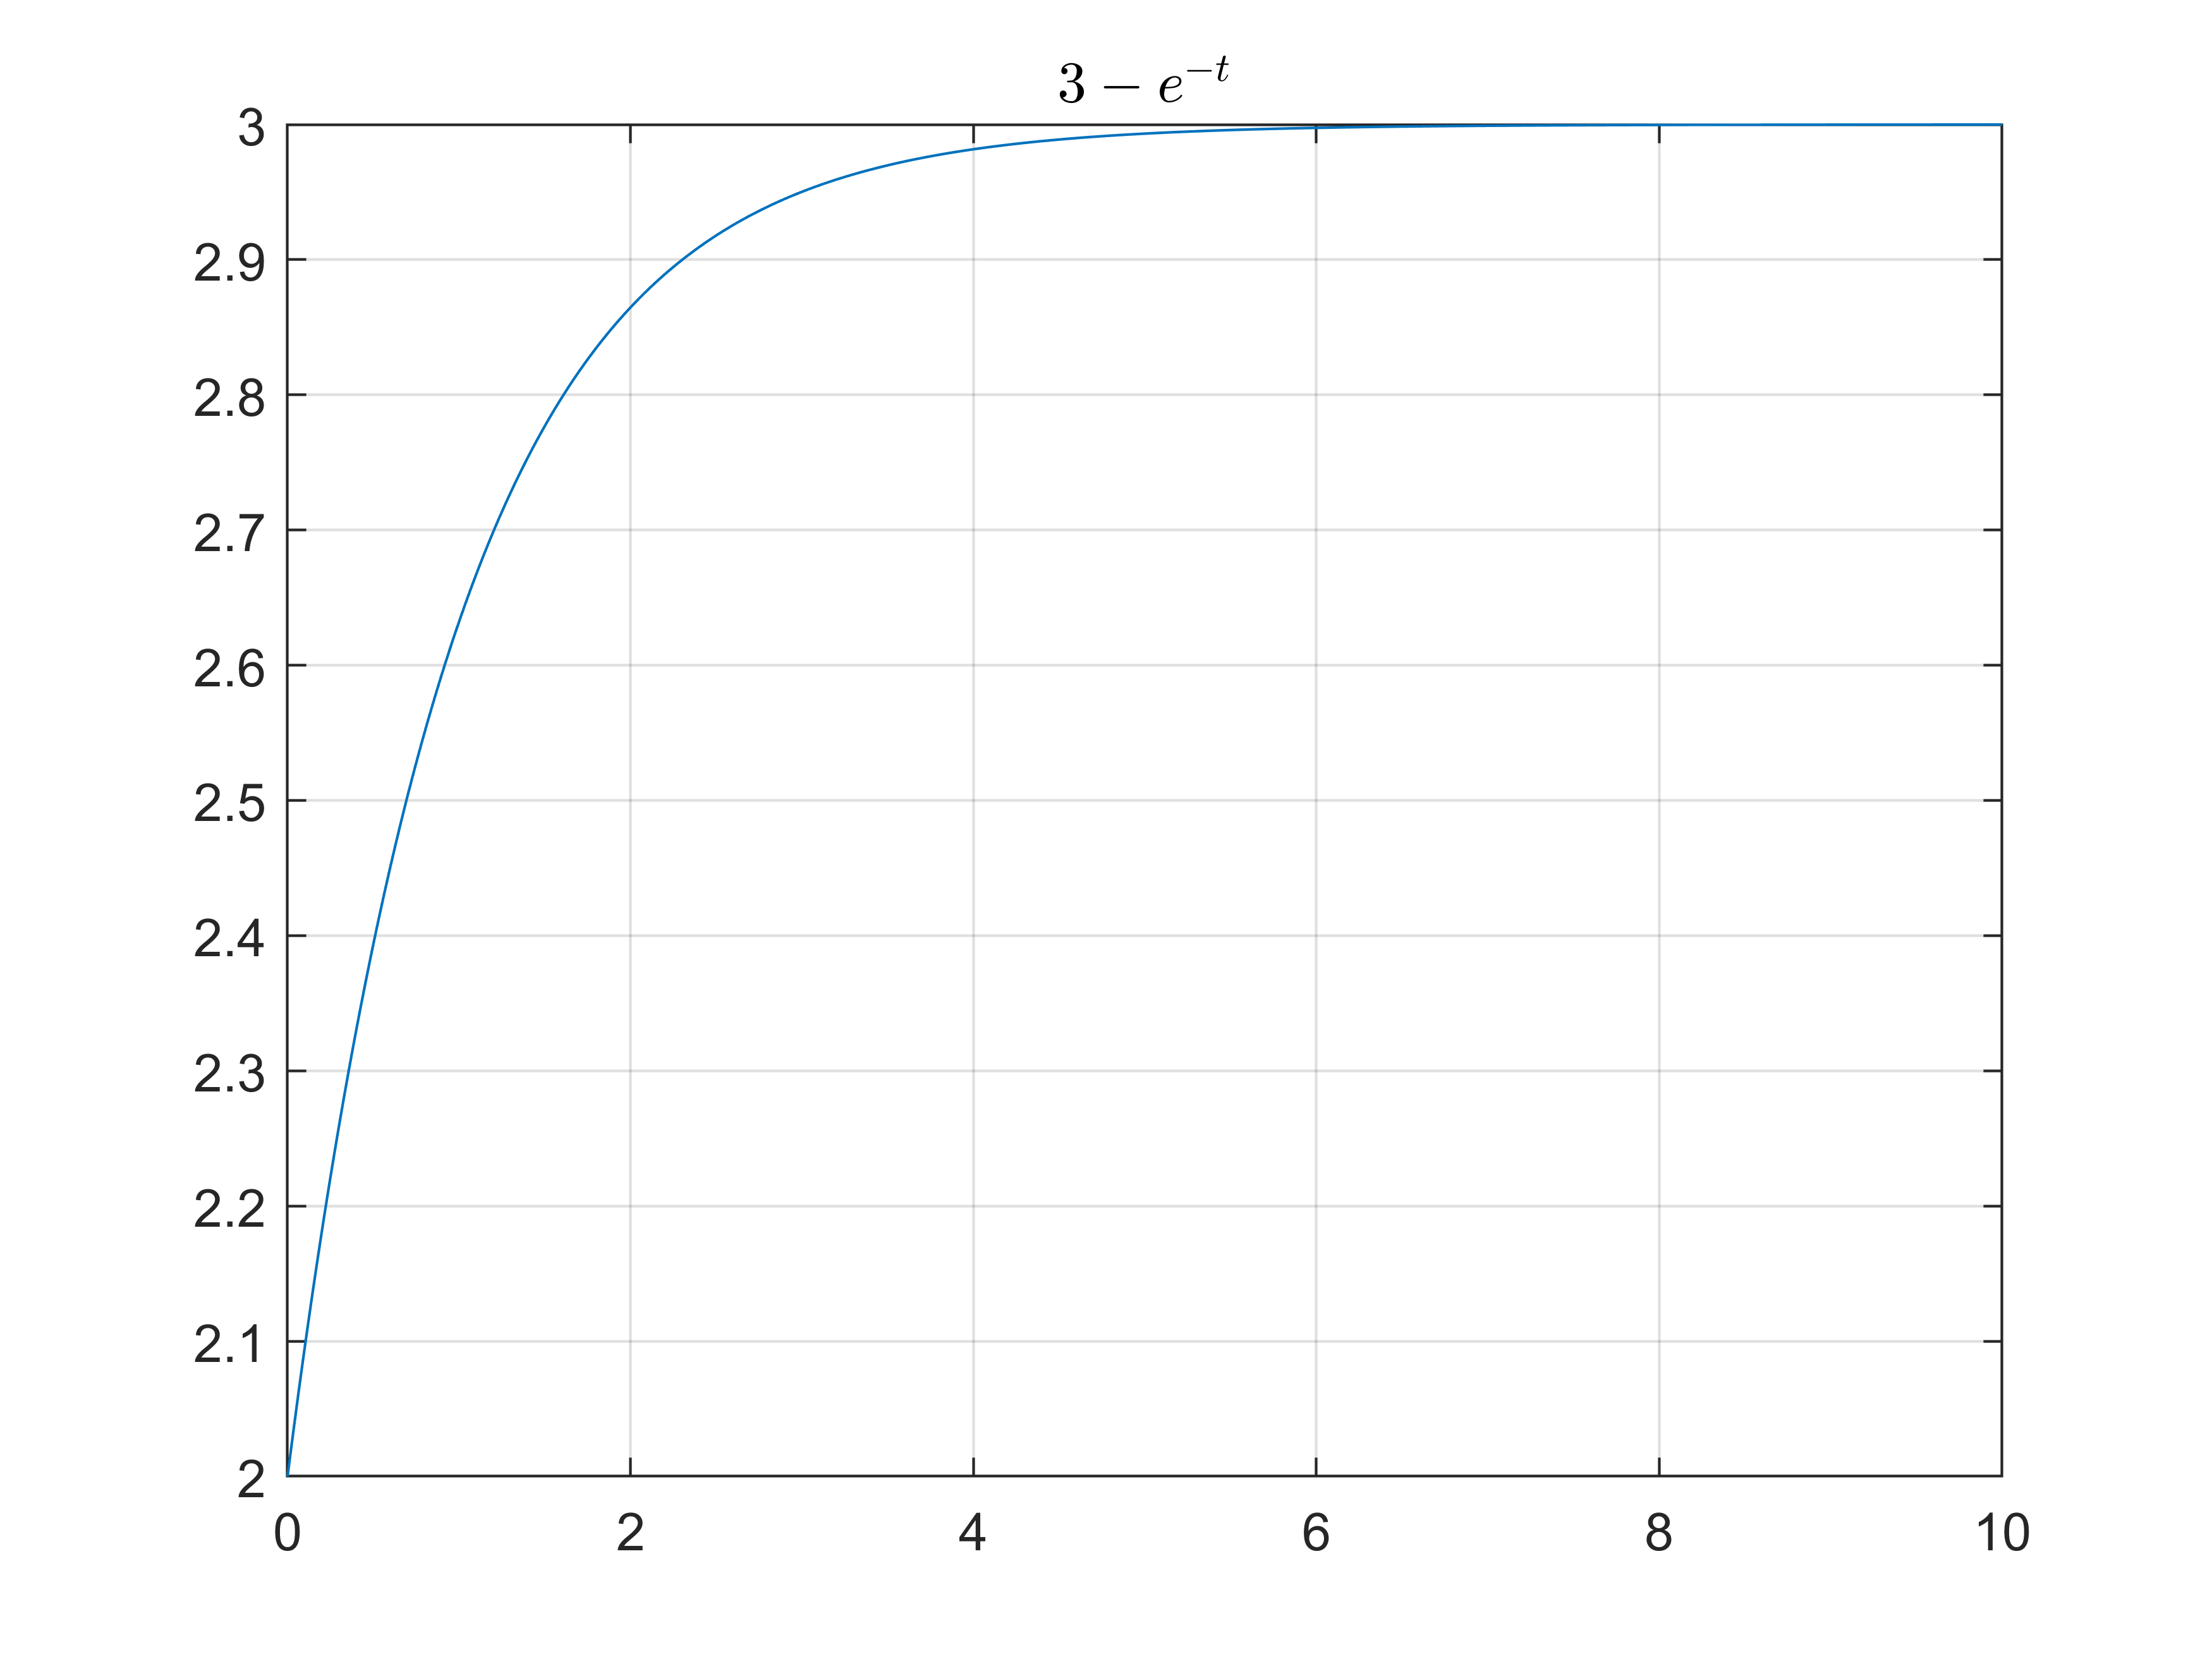
\includegraphics[scale=0.5]{8-1-1.png}
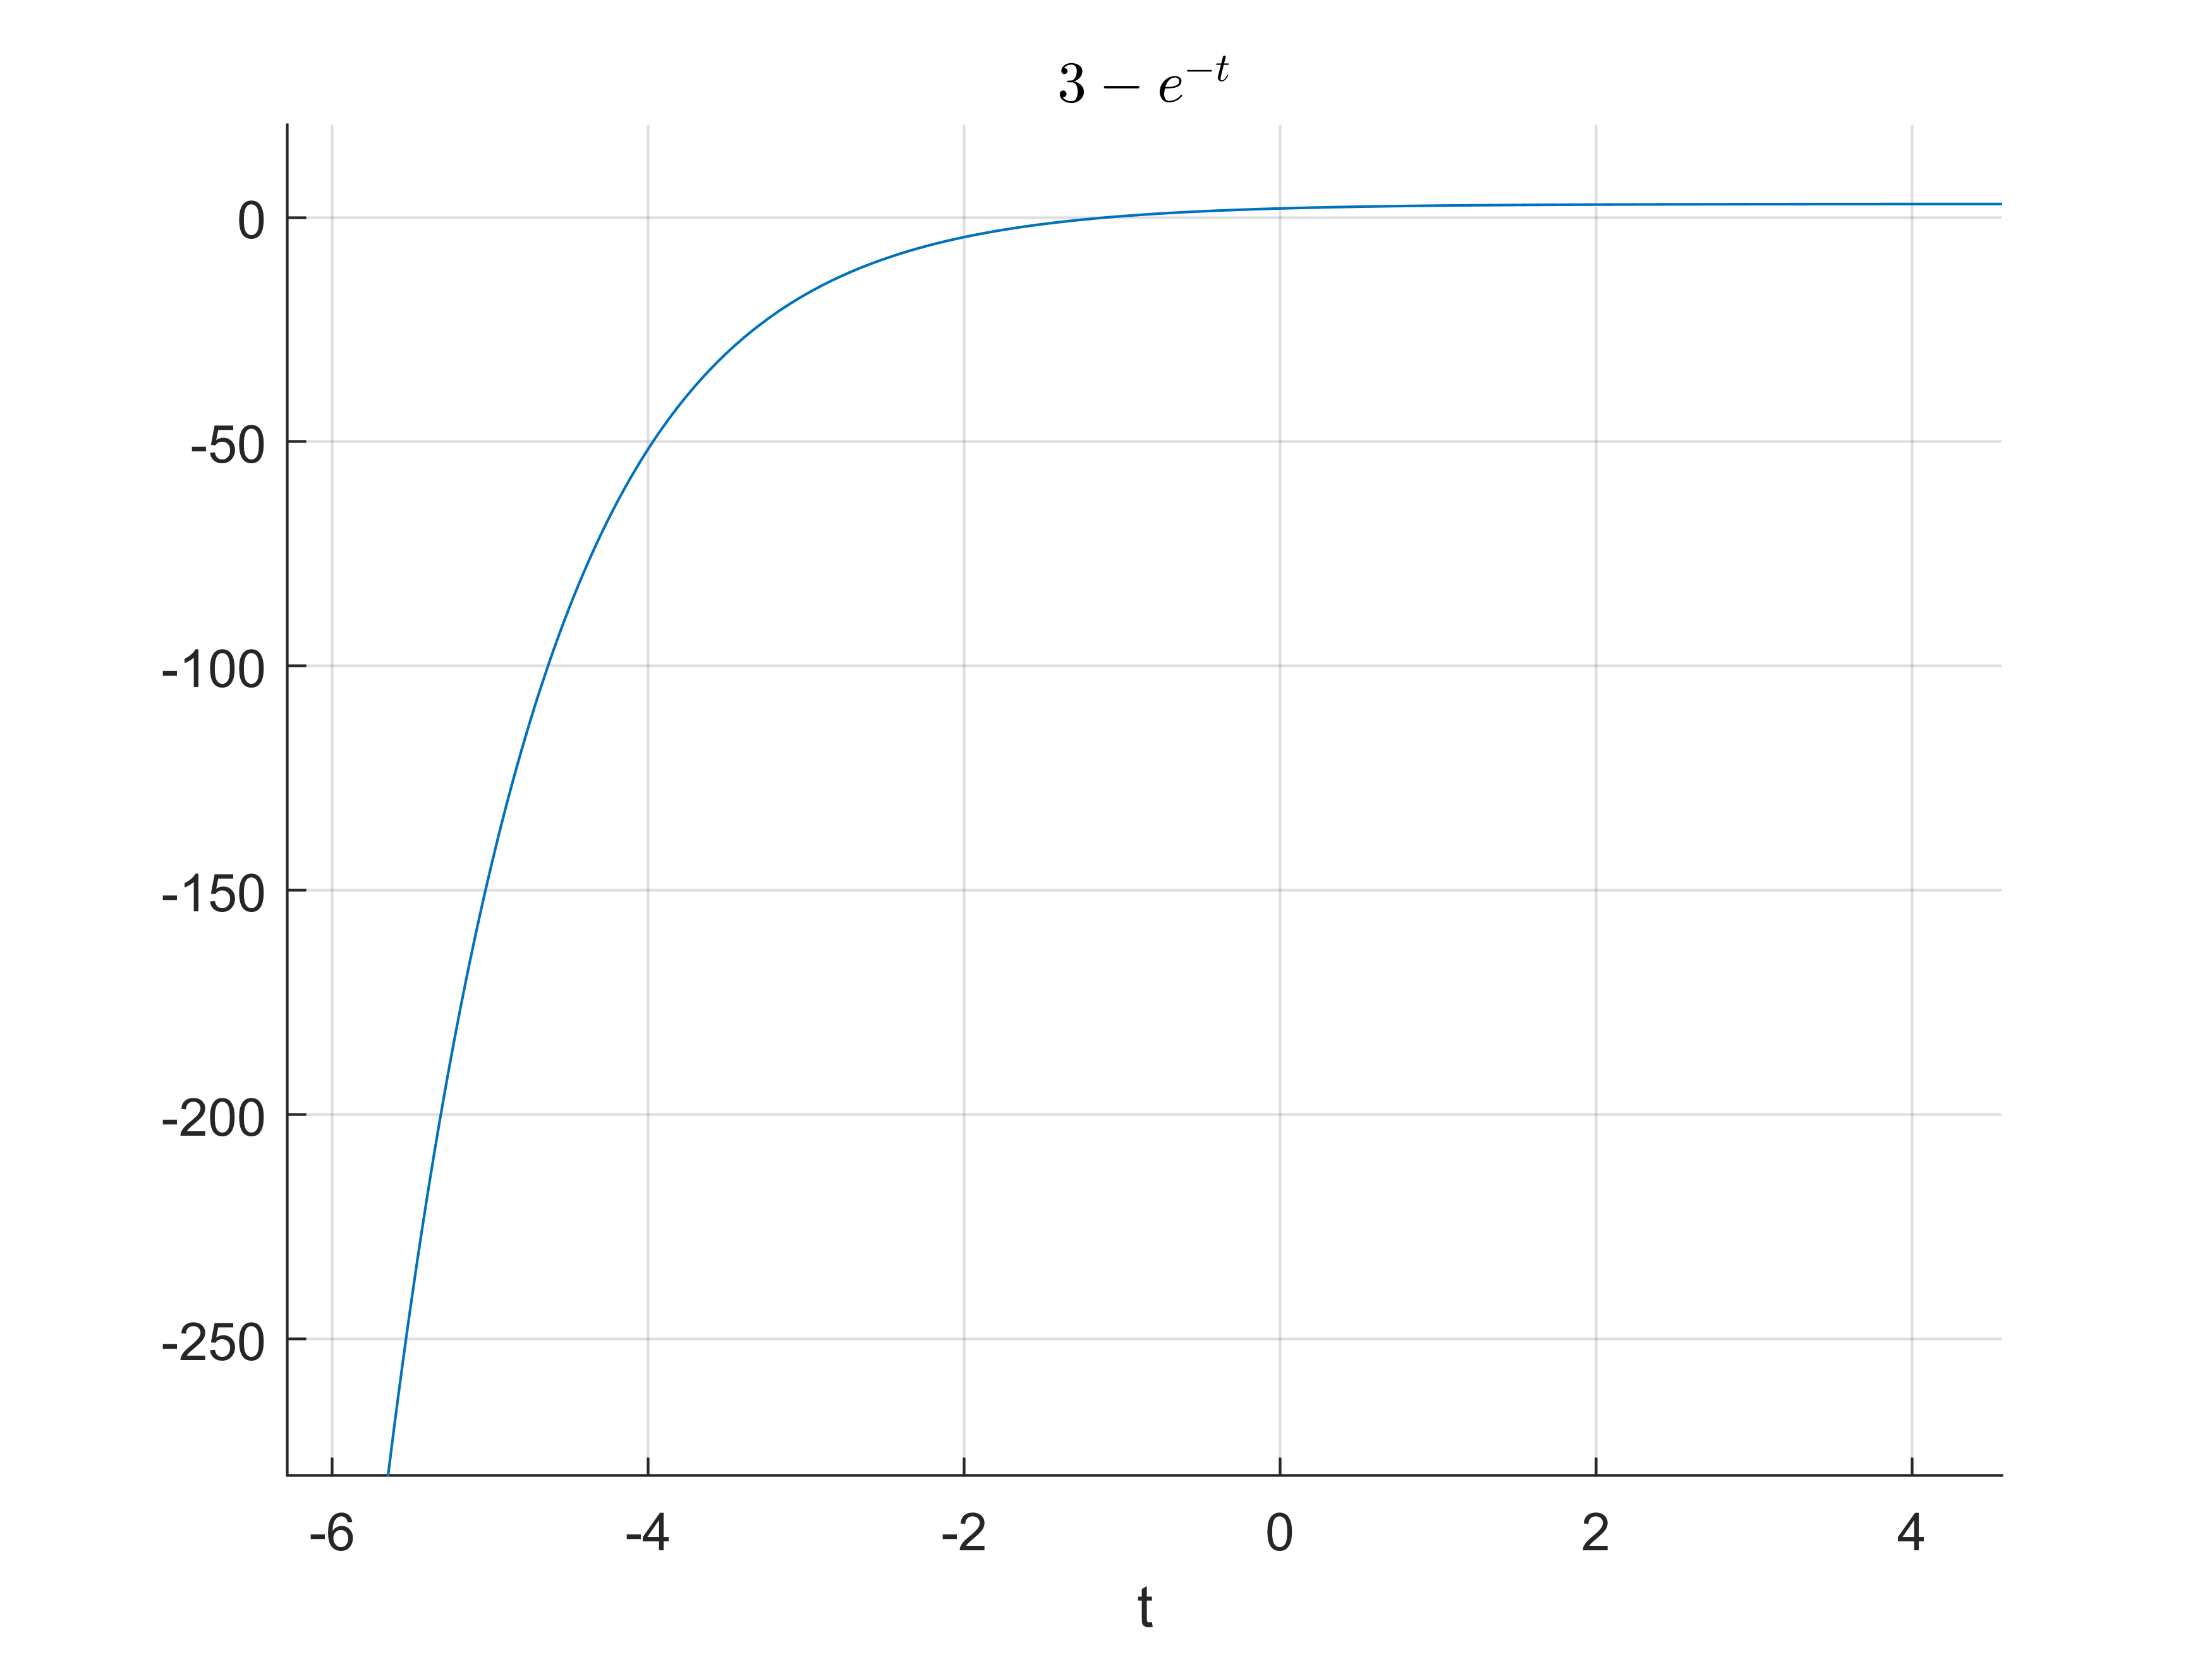
\includegraphics[scale=0.5]{8-1-2.png}\\
\textbf{Question 2}\\
\begin{lstlisting}
    clear all;
    t=0:0.01:3;
    plot(t,3*exp(-2*t)+5*exp(-t));
    hold on;
    grid on;
    title('$3e{-2*t}+5e{-t}$','Interpreter','Latex');
    hold off;
    figure(2)
    grid on;
    hold on;
    t=sym('t');
    f=sym(3*exp(-2*t)+5*exp(-t));
    ezplot(f,[0,3]);
    title('$3e{-2*t}+5e{-t}$','Interpreter','Latex');    
\end{lstlisting}
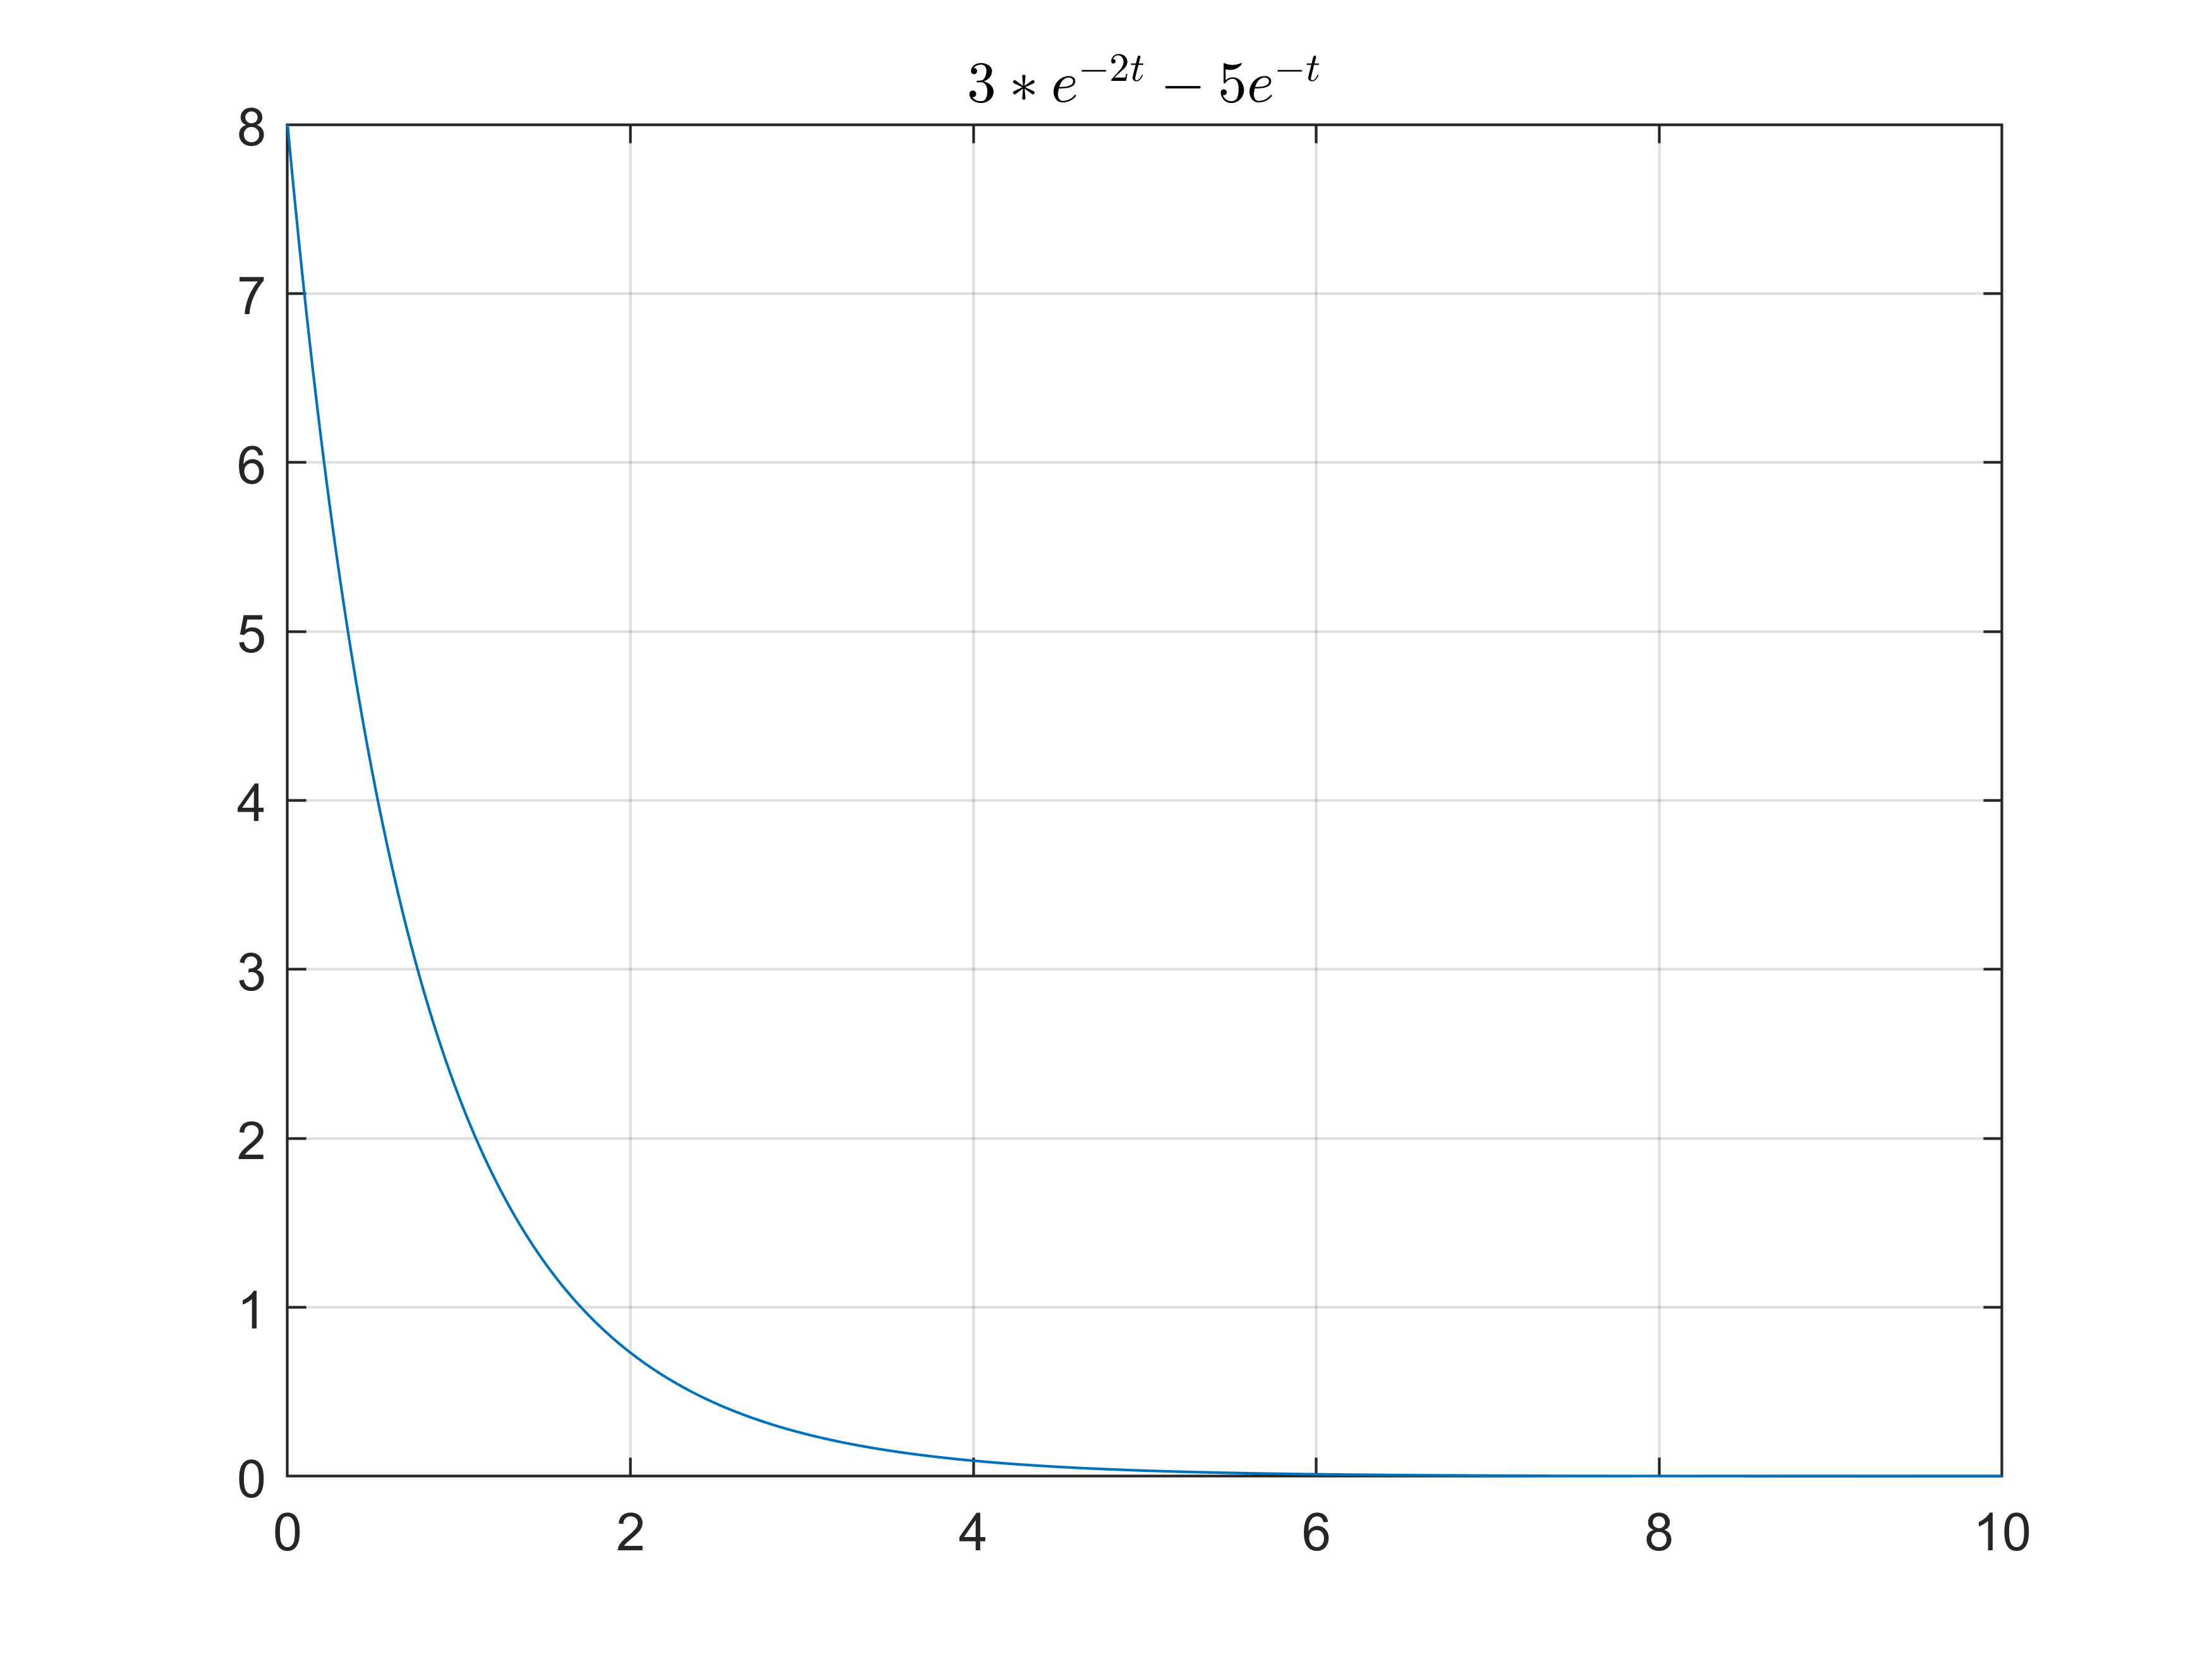
\includegraphics[scale=0.5]{8-2-1.png}
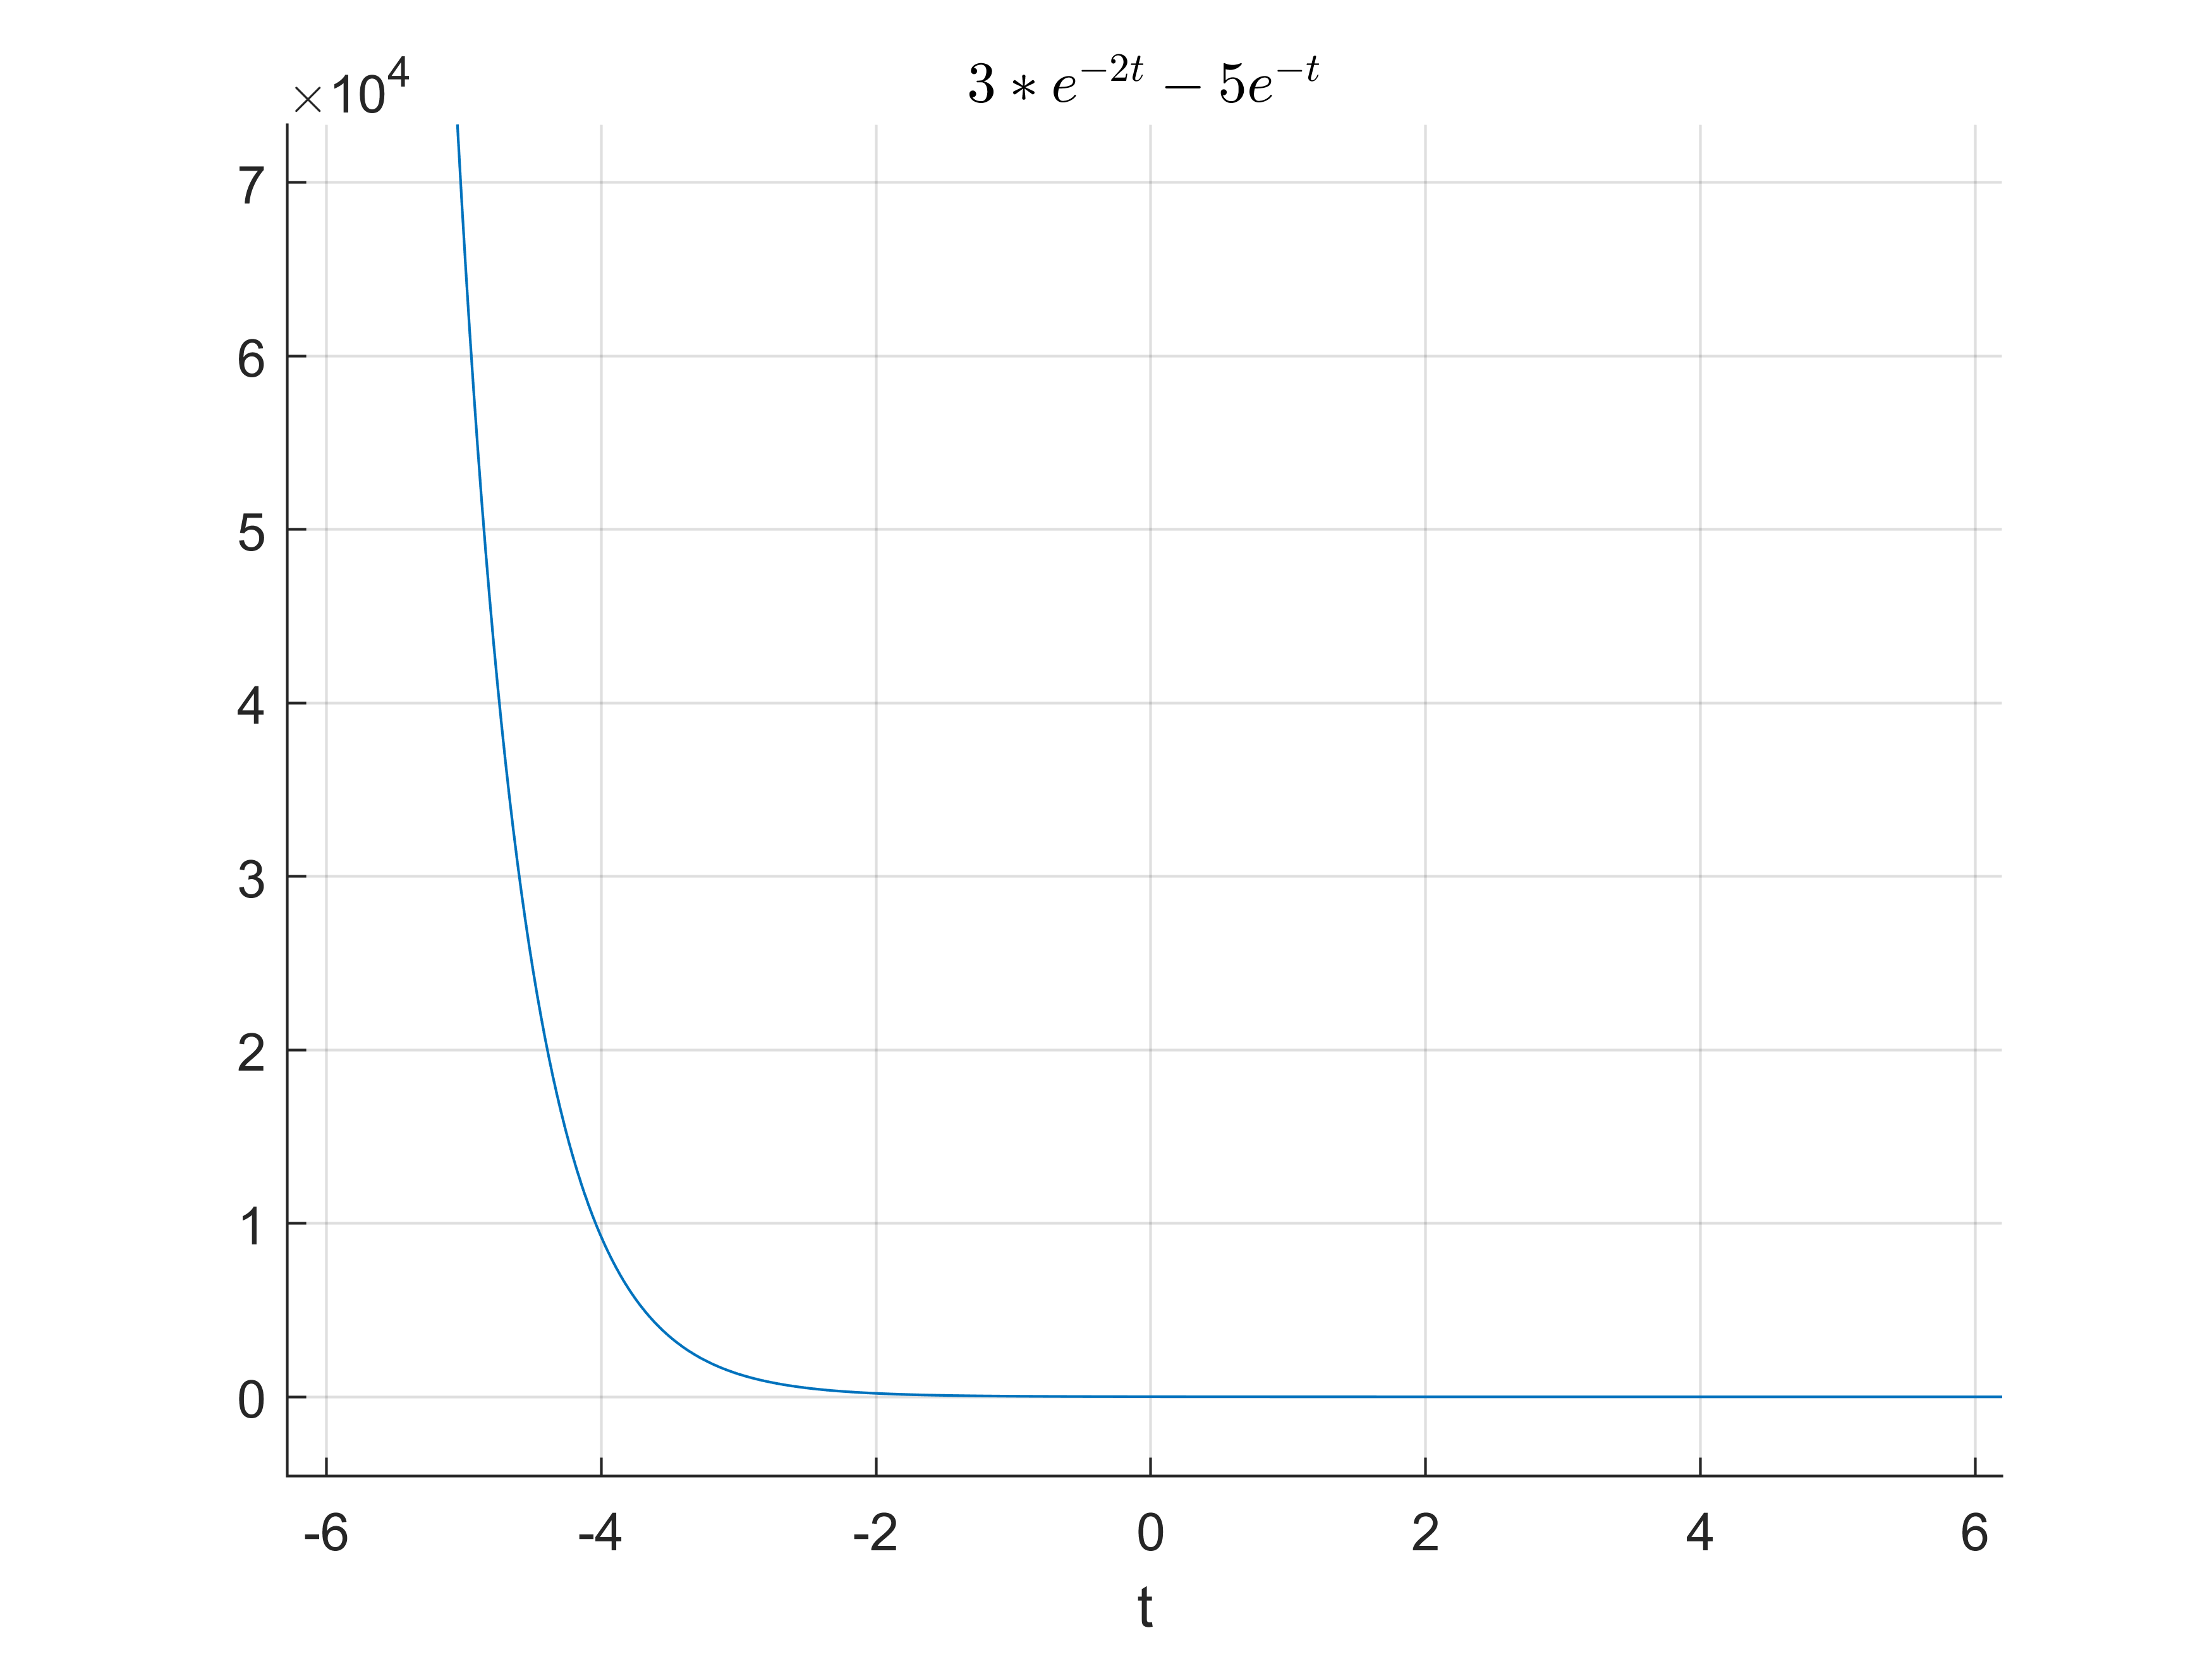
\includegraphics[scale=0.5]{8-2-2.png}\\
\textbf{Question 3}\\
\begin{lstlisting}
    clear all;
    t=0:0.01:3;
    plot(t,exp(-t).*sin(2*pi*t));
    hold on;
    grid on;
    title('$e^{-t}sin(2\pi t)$','Interpreter','Latex');
    hold off;
    figure(2)
    grid on;
    hold on;
    t=sym('t');
    f=sym(exp(-t)*sin(2*pi*t));
    ezplot(f,[0,3]);
    title('$e^{-t}sin(2\pi t)$','Interpreter','Latex'); 
\end{lstlisting}
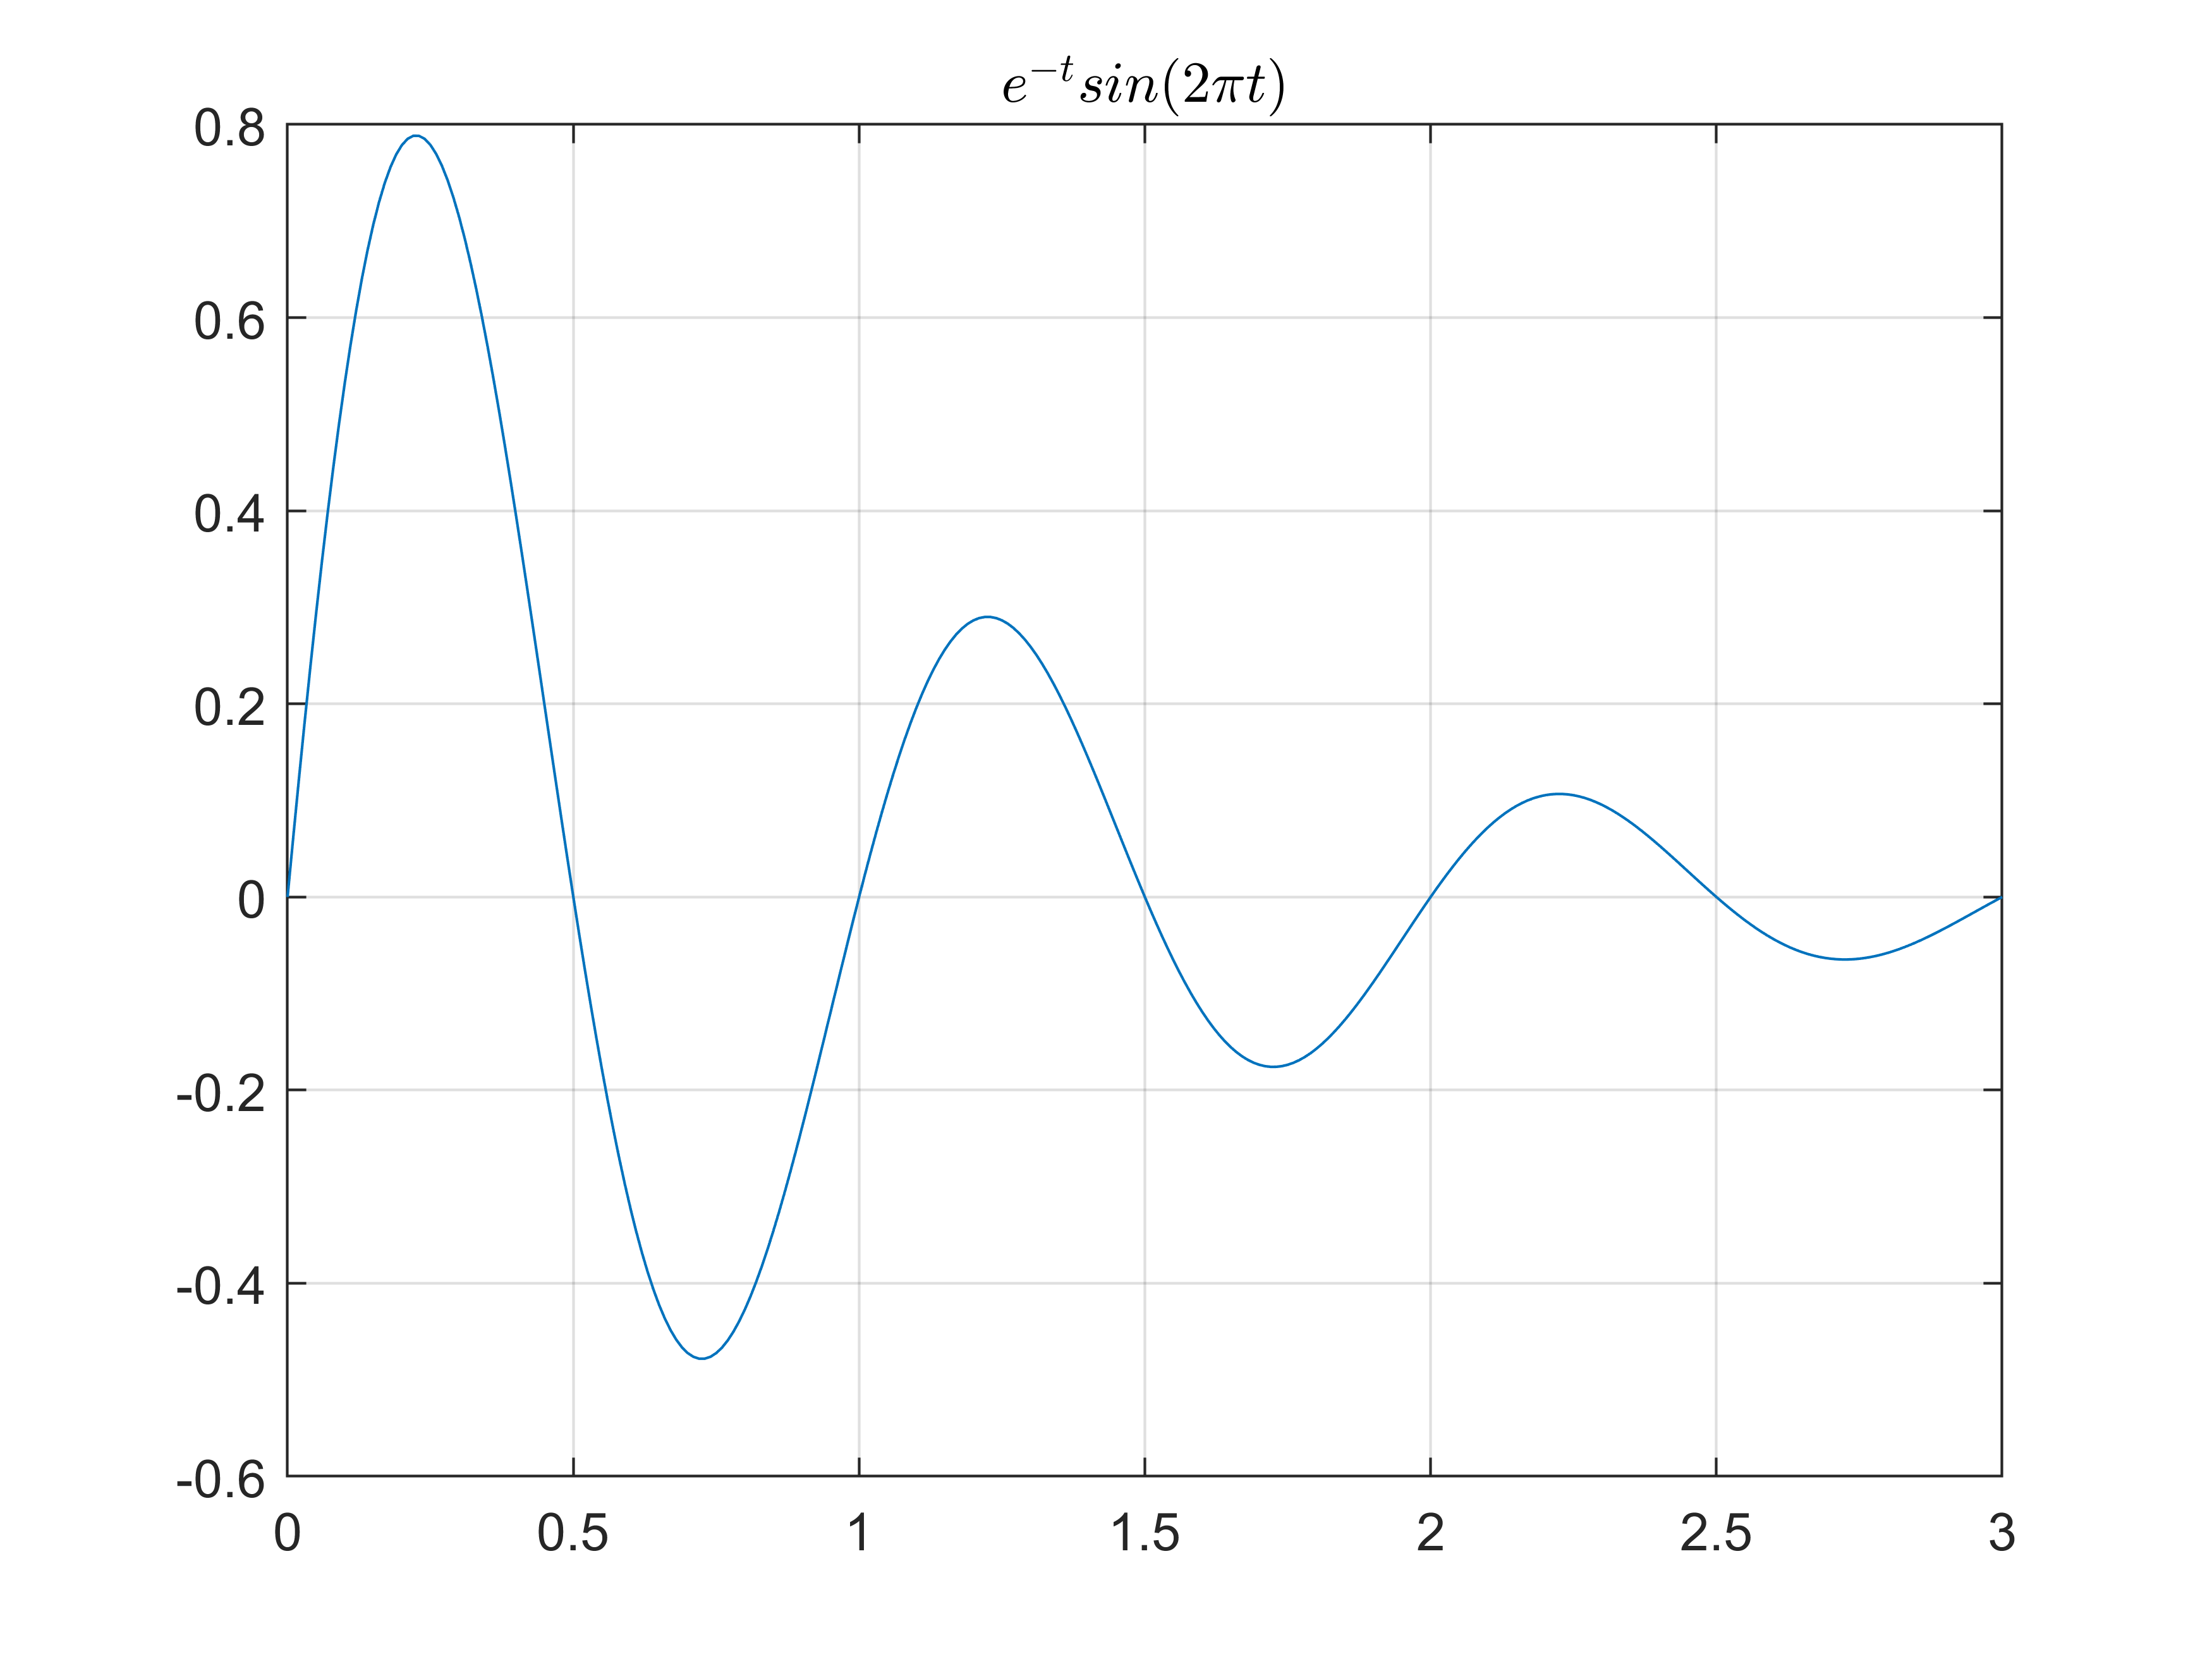
\includegraphics[scale=0.5]{8-3-1.png}
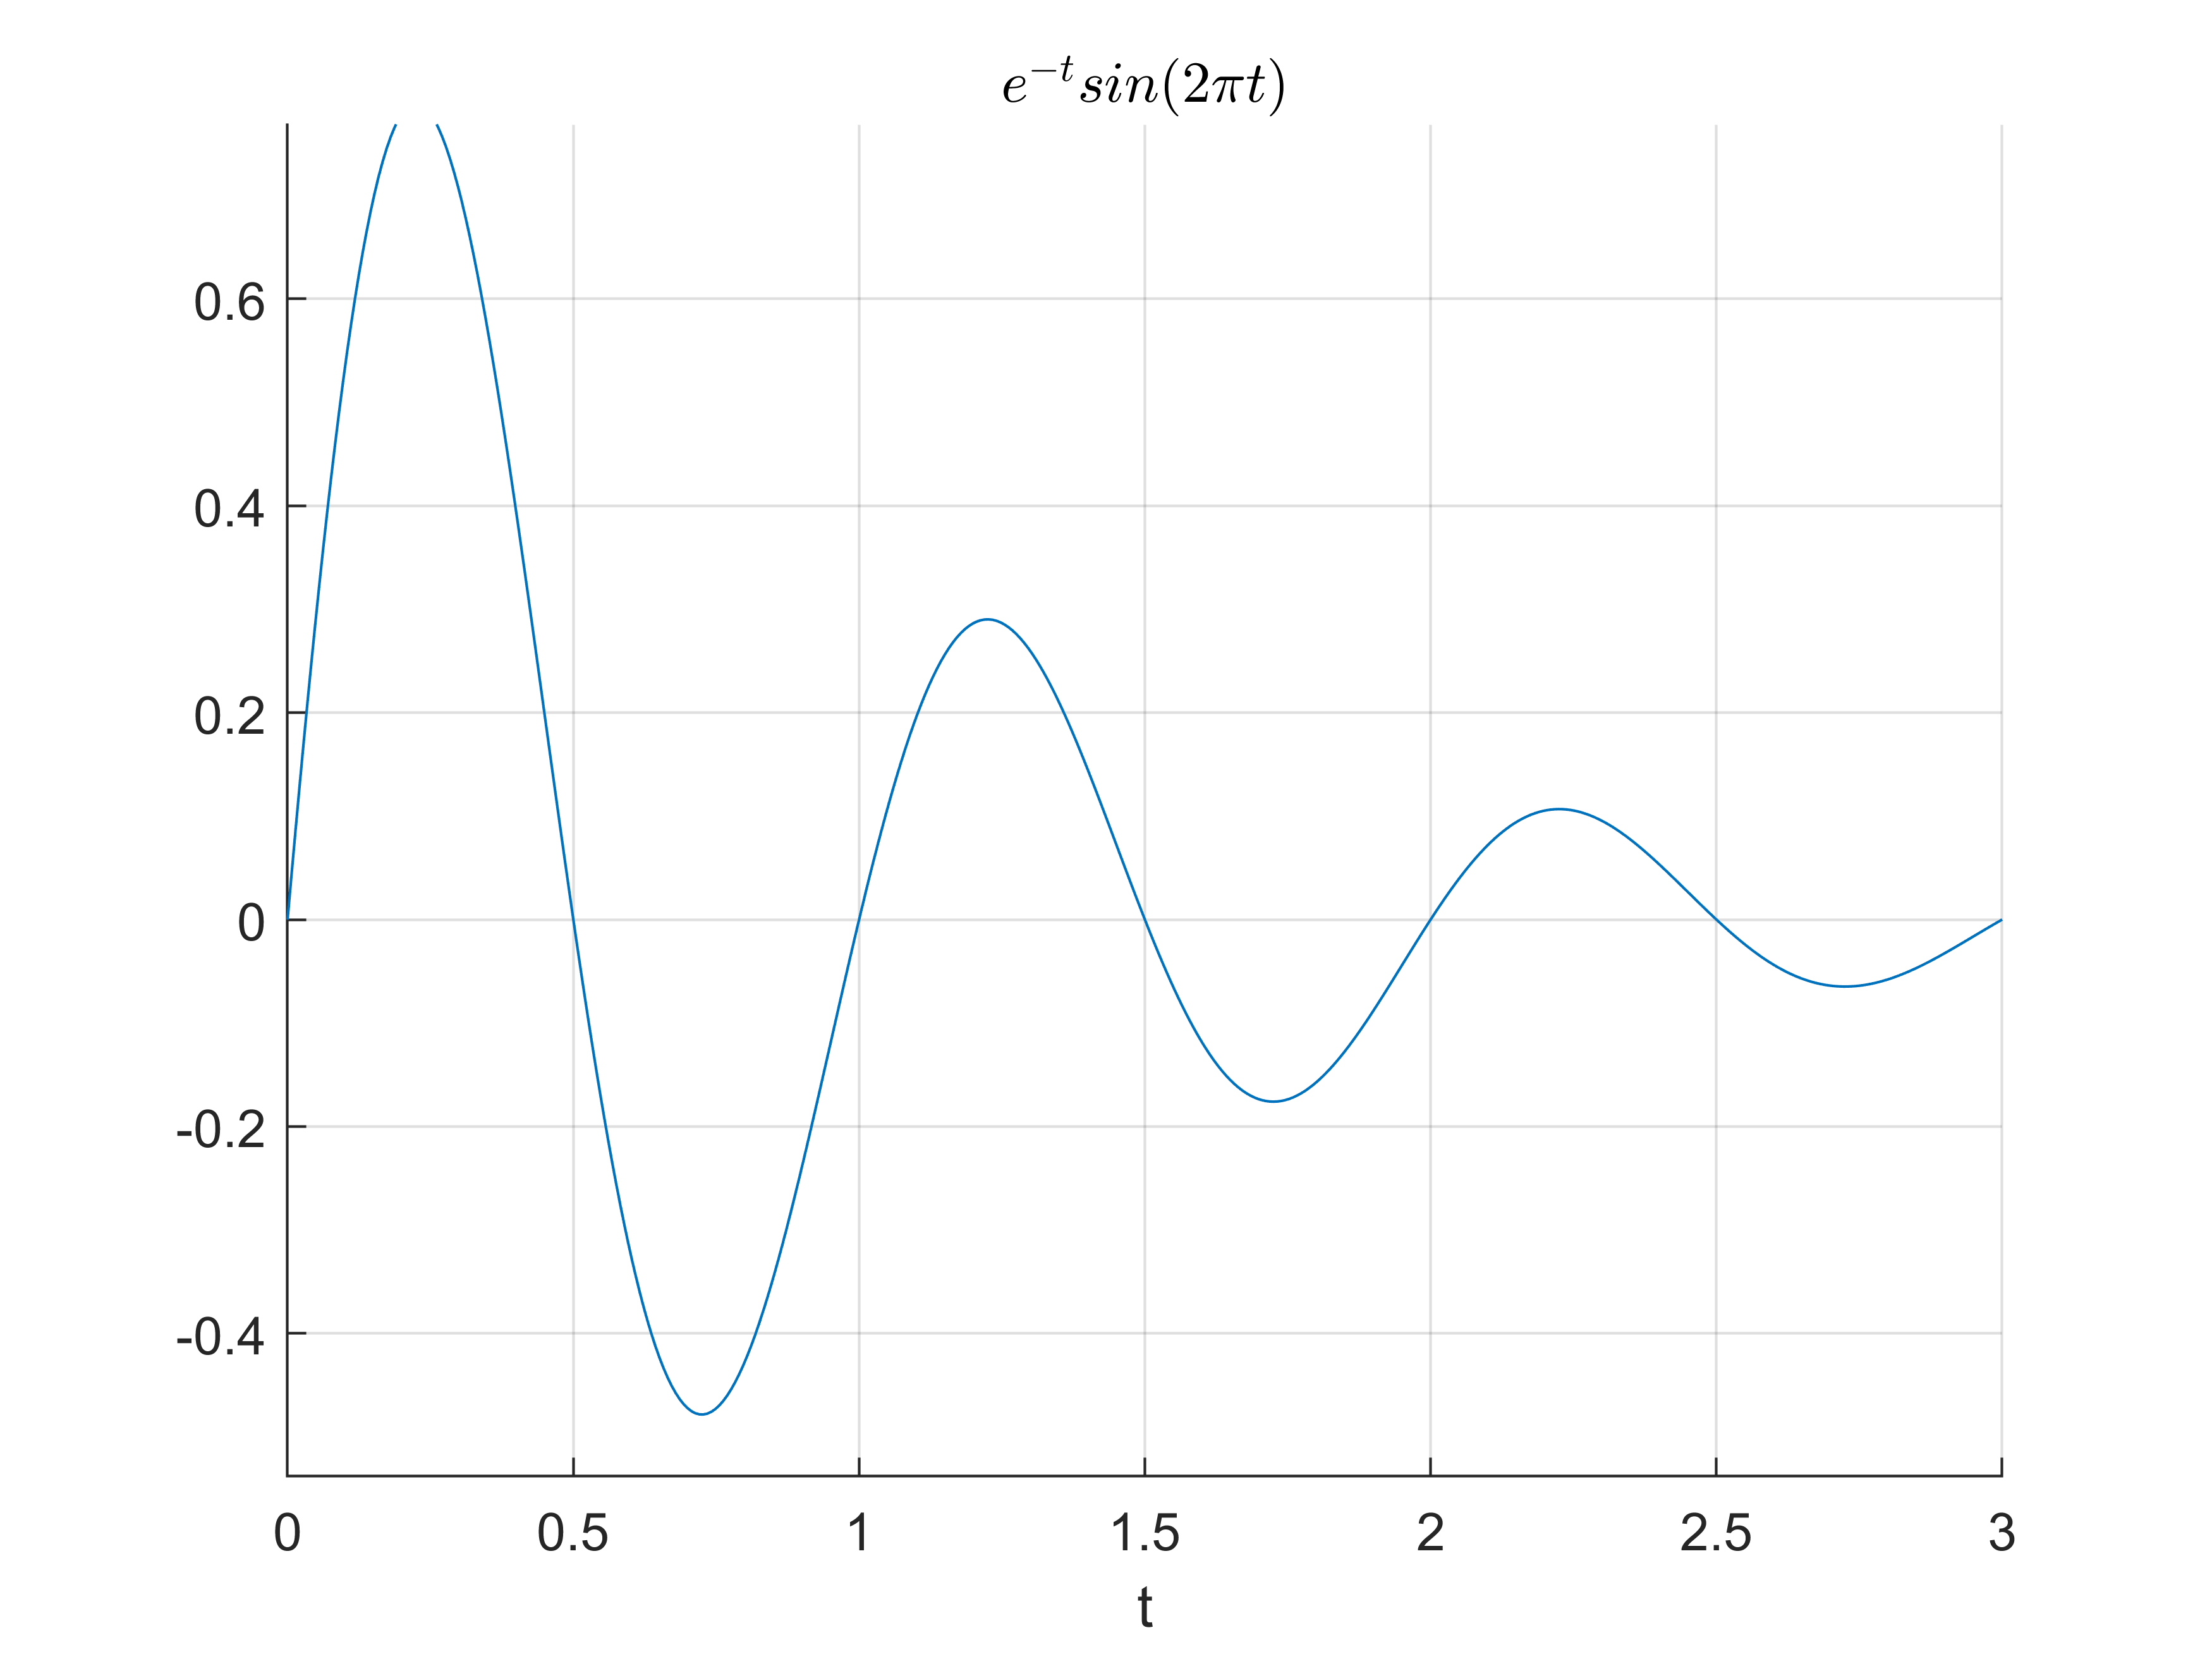
\includegraphics[scale=0.5]{8-3-2.png}\\
\textbf{Question 4}\\
\begin{lstlisting}
    clear all;
    t=-7:0.01:7;
    a=2
    plot(t,sinc(a*t/pi));
    hold on;
    grid on;
    title('$Sa(at)$','Interpreter','Latex');
    hold off;
    figure(2)
    grid on;
    hold on;
    t=sym('t');
    f=sym(sinc(a*t/pi));
    ezplot(f);
    title('$Sa(at)$','Interpreter','Latex');
\end{lstlisting}
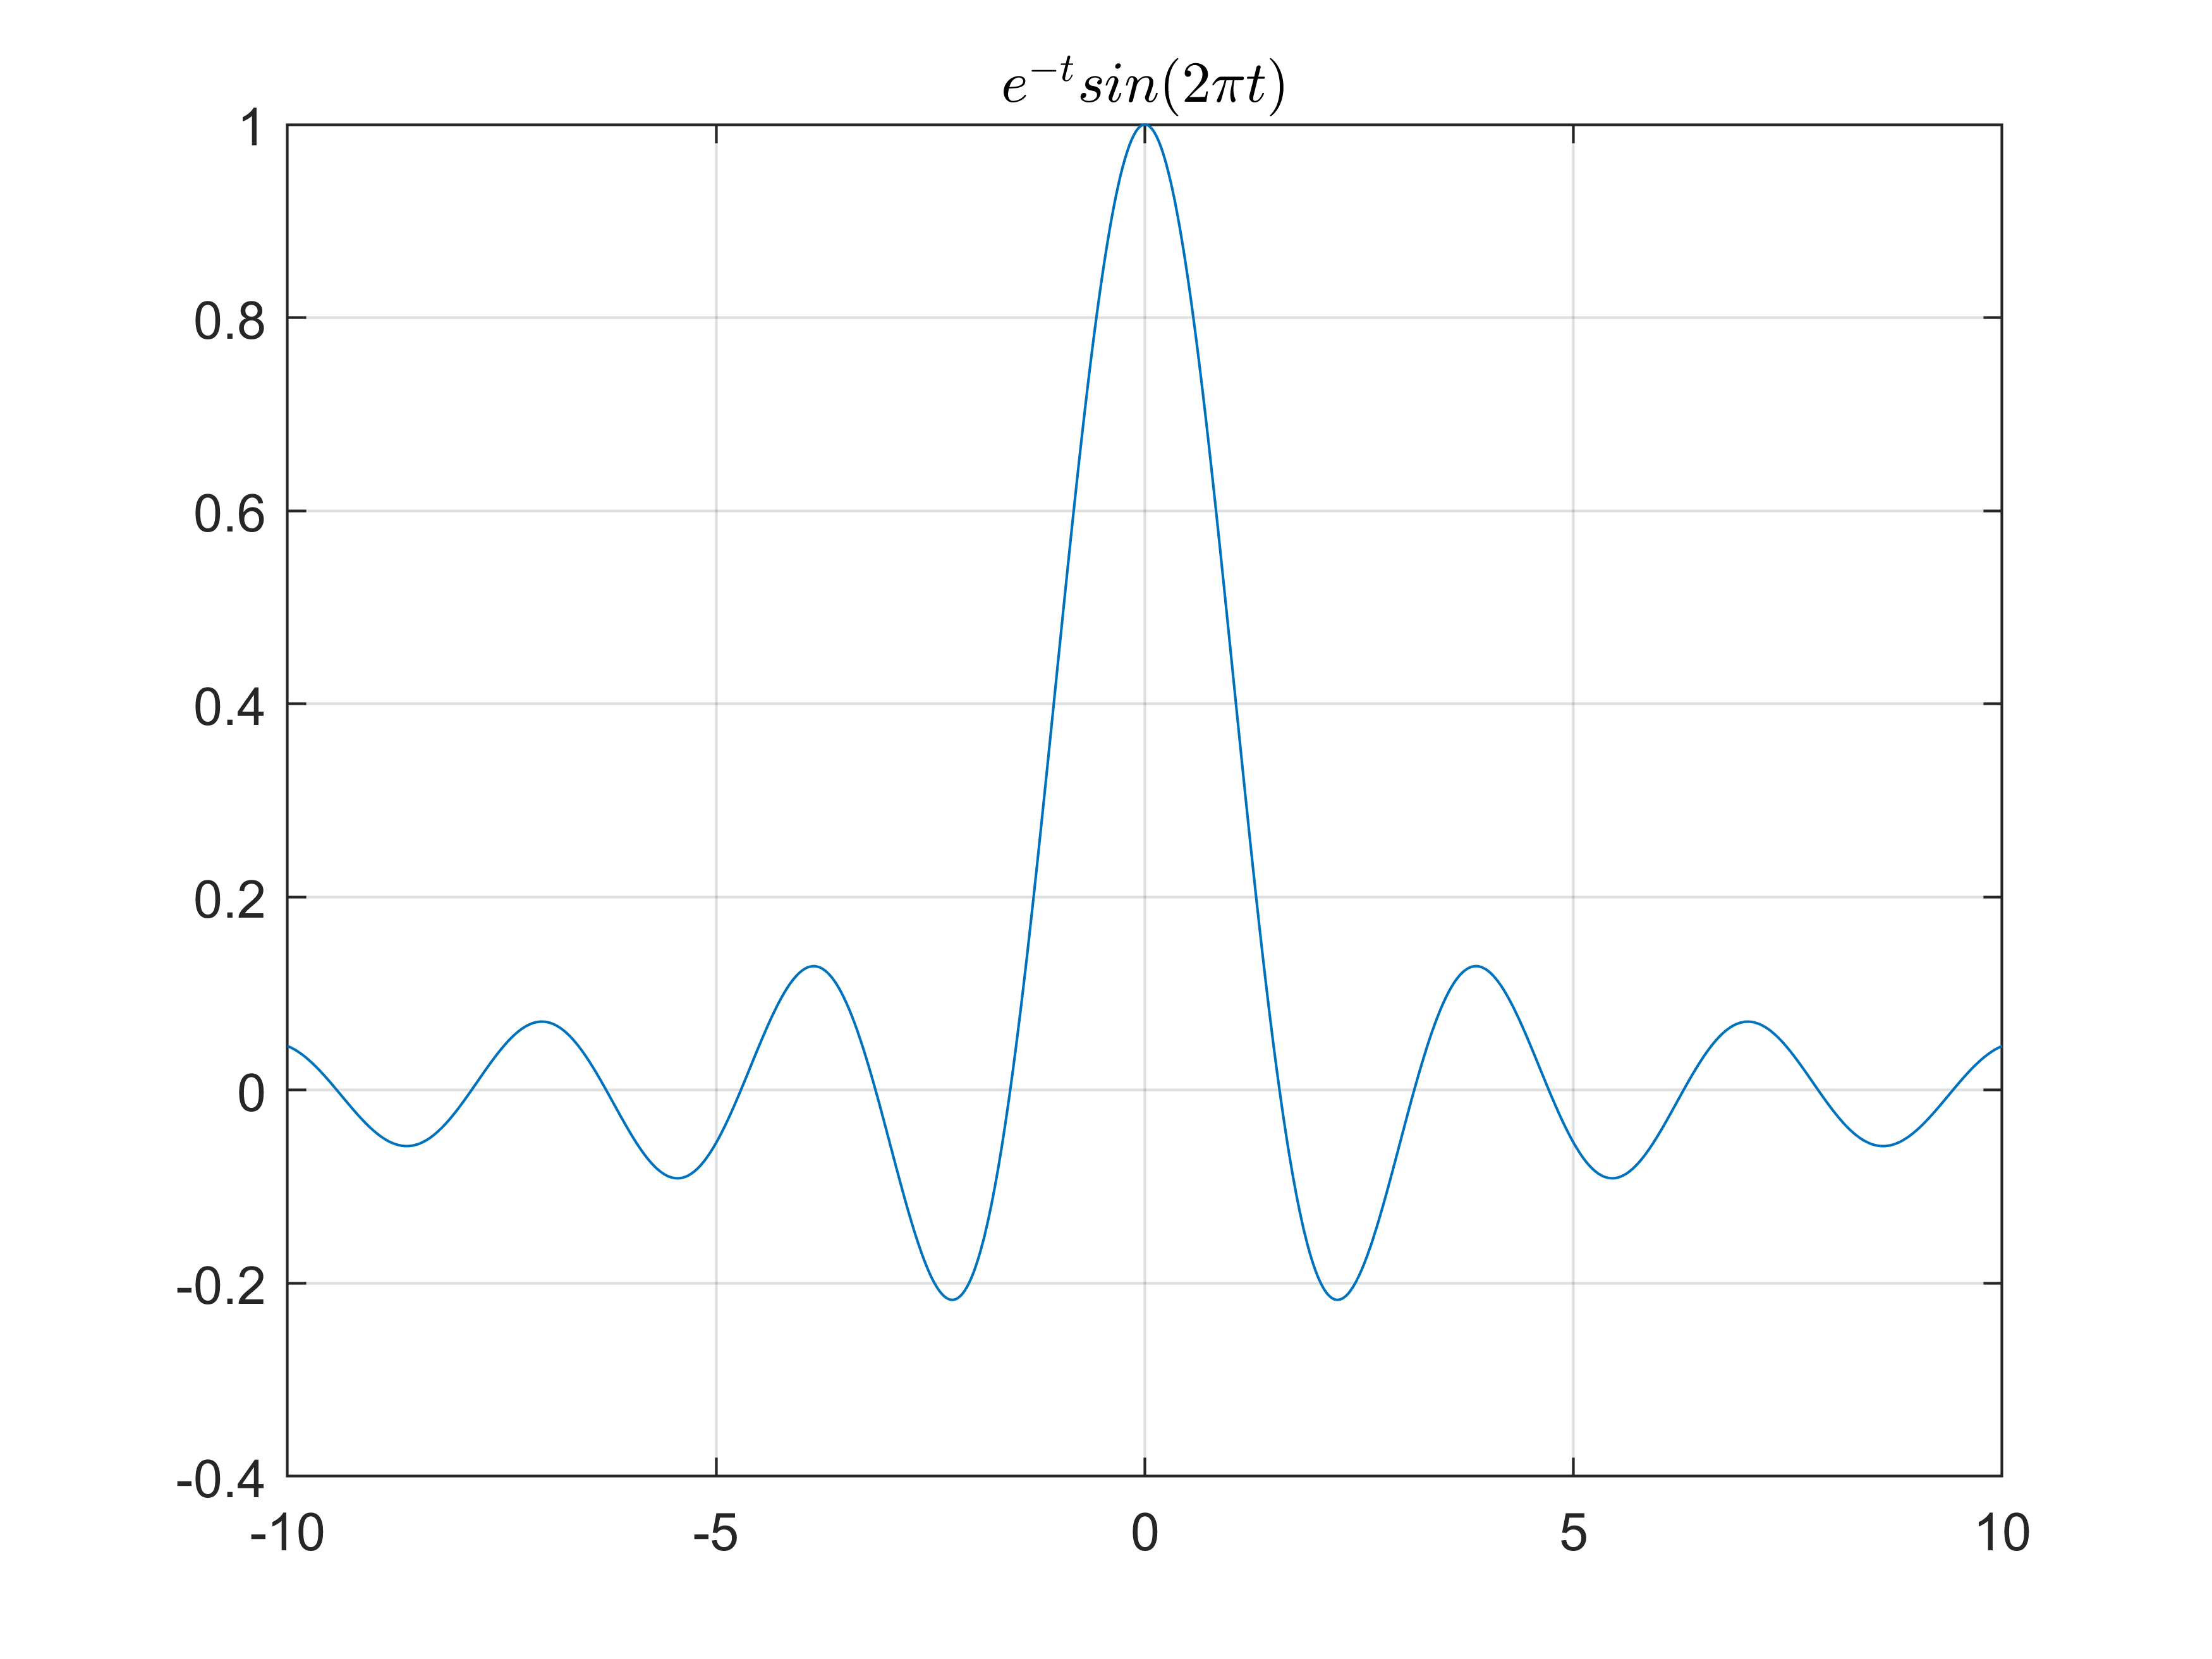
\includegraphics[scale=0.5]{8-4-1.png}
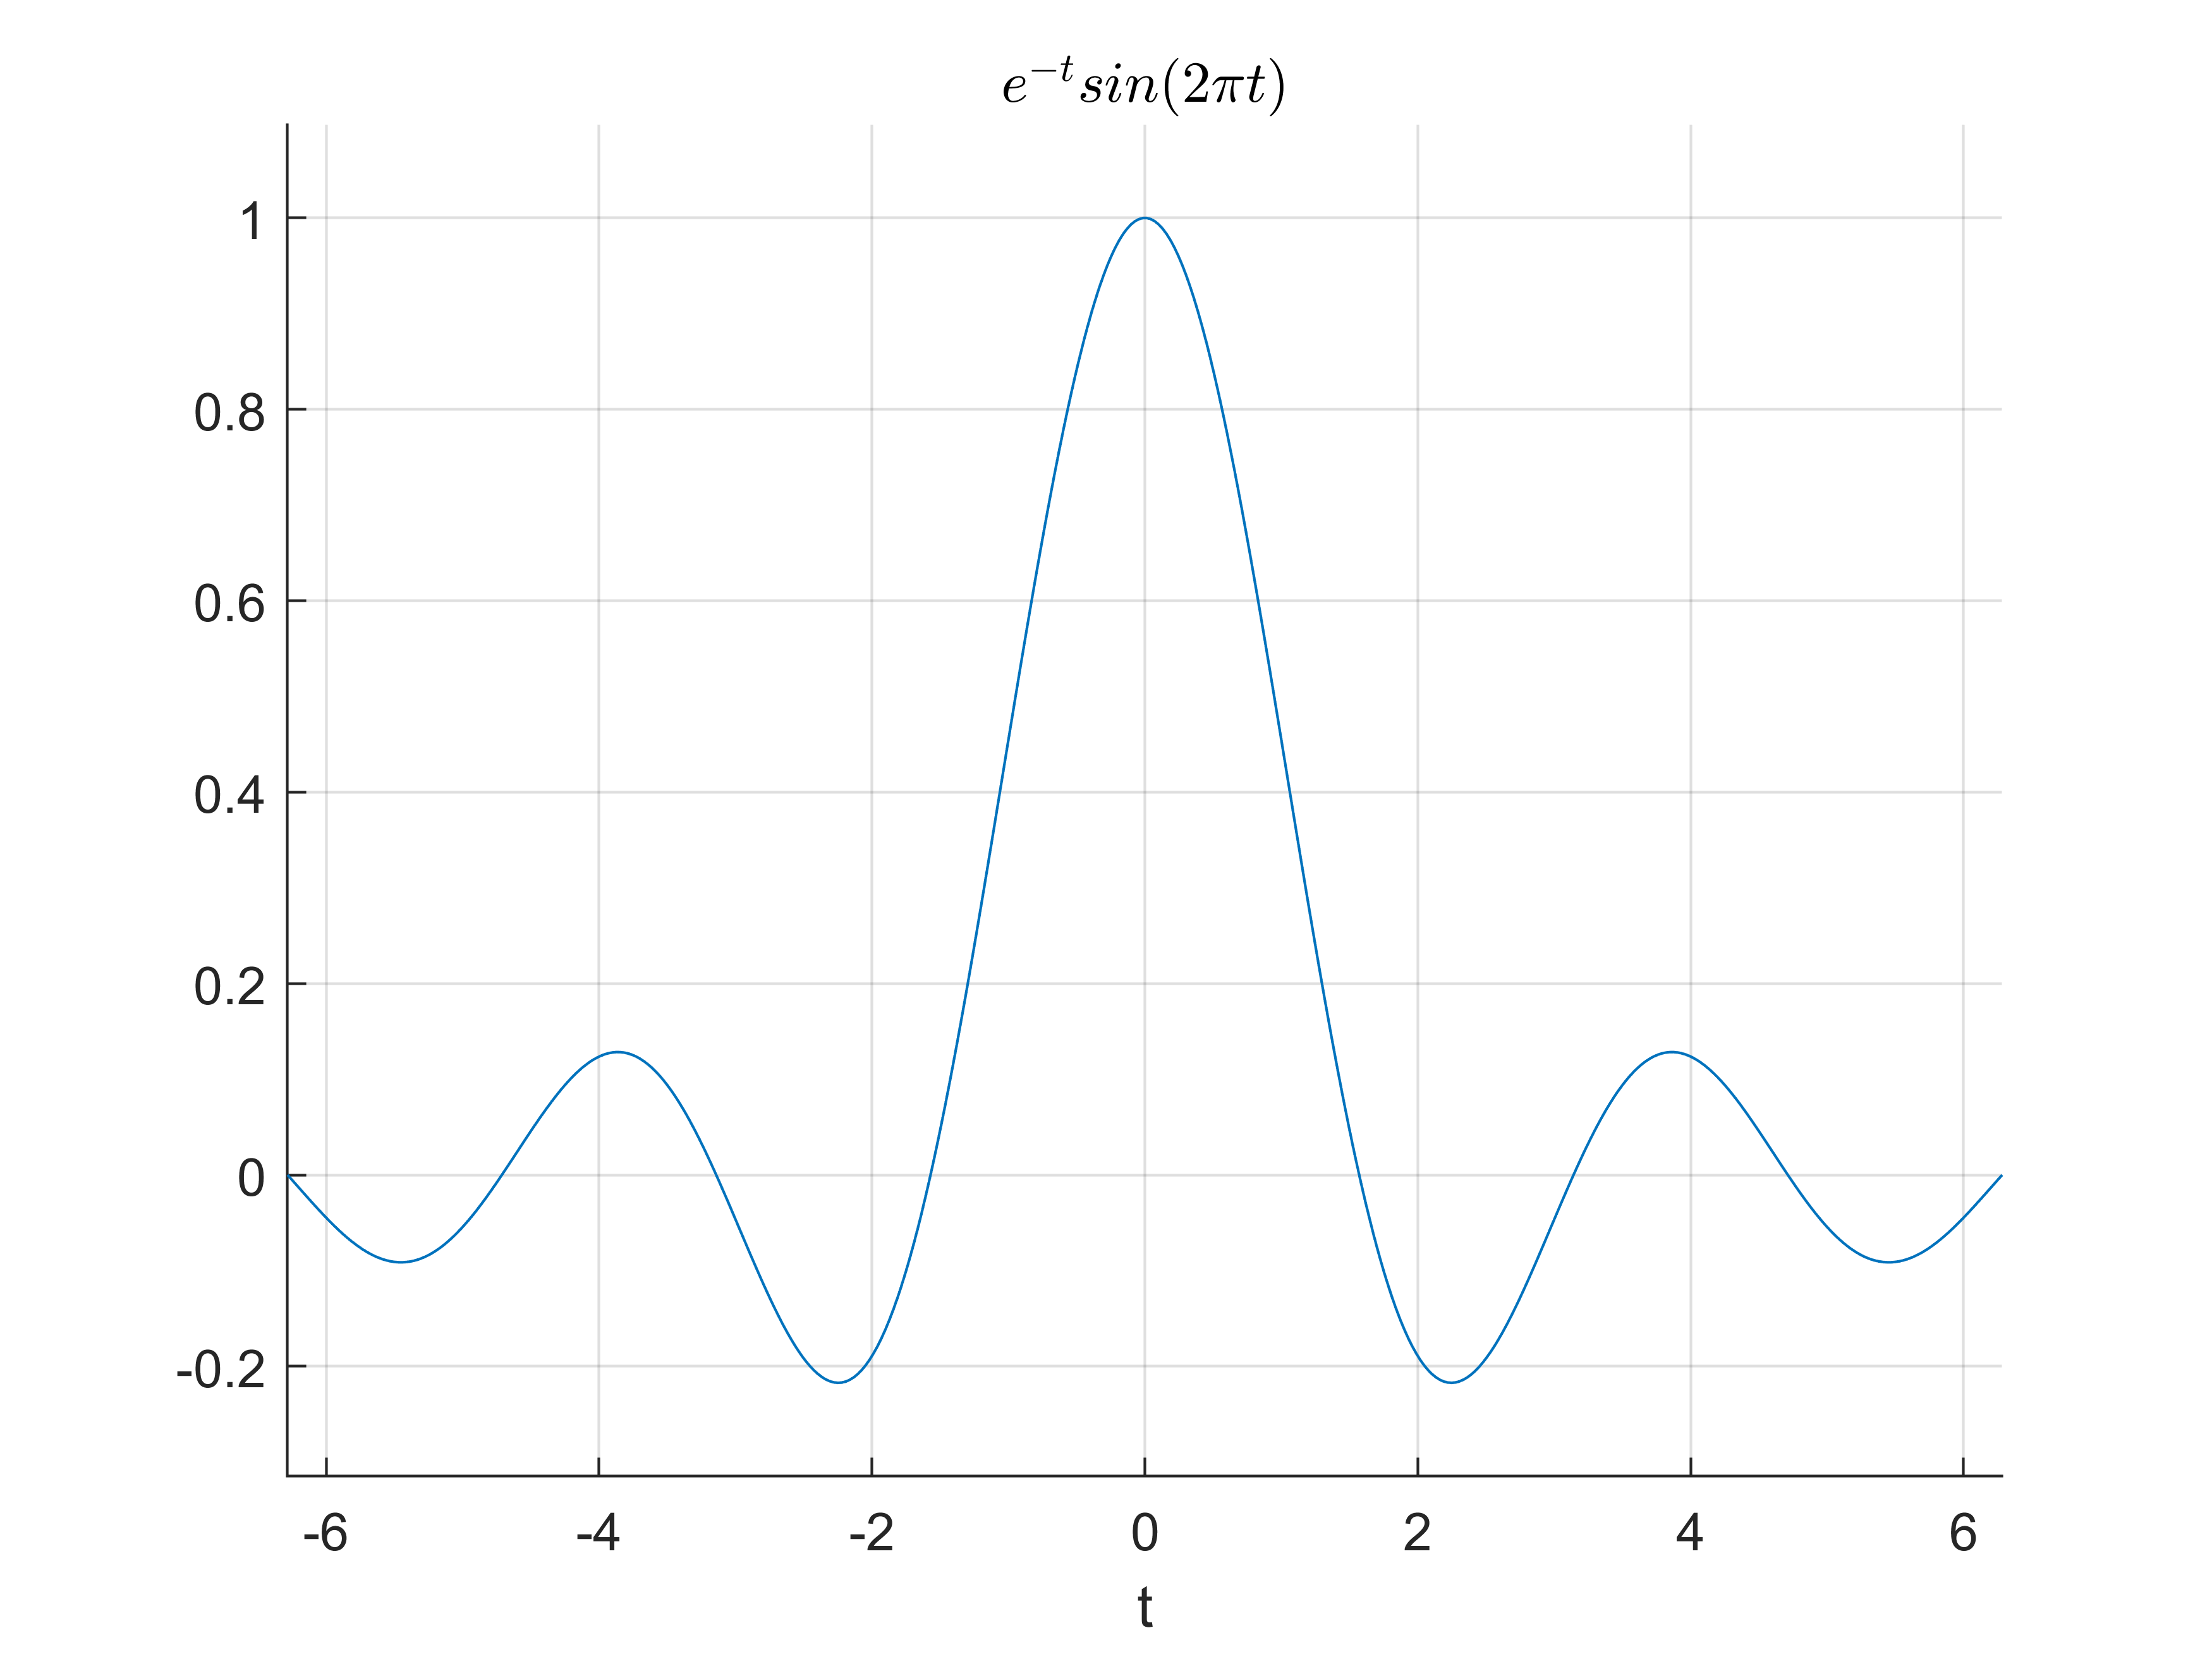
\includegraphics[scale=0.5]{8-4-2.png}\\
\end{document}